% FONTE TEMA https://github.com/matze/mtheme
\documentclass[aspectratio=1610]{beamer}
%\documentclass[aspectratio=1610, handout]{beamer}
\usepackage[utf8]{inputenc}
\usepackage{ragged2e}
\usepackage{xcolor}
\usepackage[italian]{babel}
\usepackage{multirow}
\usepackage{silence}
\usepackage{listings}
\definecolor{verde}{rgb}{0,0.6,0}
\definecolor{grigio}{rgb}{0.5,0.5,0.5}
\definecolor{rosa}{rgb}{0.58,0,0.82}
\definecolor{backgroud}{rgb}{0.95,0.95,0.92}
\lstdefinestyle{stilepython}{
    backgroundcolor=\color{backgroud},
    commentstyle=\color{verde},
    keywordstyle=\color{magenta},
    numberstyle=\tiny\color{grigio},
    stringstyle=\color{rosa},
    basicstyle=\ttfamily\footnotesize,
    breakatwhitespace=false,
    numbers=left,
    numbersep=5pt,
    showspaces=false,
    showstringspaces=false,
    showtabs=false,
    literate=
    {à}{{\'a}}1
    {è}{{\'e}}1
    {ì}{{\'i}}1
    {ò}{{\'o}}1
    {ù}{{\'u}}1
}
\lstset{style=stilepython}

\WarningFilter{beamer}{}
\WarningFilter{metropolis}{}
\usetheme[progressbar=frametitle,titleformat=smallcaps]{metropolis}
\setbeamertemplate{frame numbering}[fraction]
\setbeamercovered{dynamic}
\definecolor{rosso}{RGB}{255, 0, 0}
\definecolor{giallo}{RGB}{254,212,23}
\hypersetup{colorlinks=true,linkcolor=black,urlcolor=rosso}
\setbeamercolor{palette primary}{fg=black, bg=giallo}
\setbeamercolor{background canvas}{bg=white}
\setbeamercolor{normal text}{fg=black}
\setbeamercolor{progress bar}{fg=rosso}
\setbeamercolor{framesubtitle}{fg=rosso}
\setbeamercolor{normal text .dimmed}{fg=giallo}
\setbeamercolor{block title alerted}{fg=rosso, bg=giallo}
\setbeamerfont{caption}{size=\tiny}
\setbeamerfont{caption name}{size=\tiny}
\setlength{\abovecaptionskip}{0pt}
\makeatletter
\metroset{block=fill}
\setlength{\metropolis@progressinheadfoot@linewidth}{1pt} 
\setlength{\metropolis@progressonsectionpage@linewidth}{1pt}
\setlength{\metropolis@titleseparator@linewidth}{1pt}
\makeatother

\title{STRUTTURE DI CONTROLLO}
\subtitle{Selezione e cicli iterativi}
\date{}
\institute{\textit{
        Fonti:
        \begin{itemize}
            \item[-] \href{https://docs.python.org/it/3.15/tutorial/controlflow.html}{Controllo del Flusso di Esecuzione - Documentazione Ufficiale Python}
        \end{itemize}
    }
}

\begin{document}

\begin{frame}[plain, noframenumbering]
    \titlepage
\end{frame}

\section{ISTRUZIONI IF - ELSE - ELIF}

\begin{frame}[fragile]{ISTRUZIONE IF}
    \begin{alertblock}{DEFINIZIONE}
        \begin{minipage}{0.98\linewidth}
            \justifying
            L'istruzione \textbf{if} permette di eseguire un blocco di codice solo se una 
            condizione è verificata. Se la condizione è falsa, il blocco di codice viene saltato.\\
\begin{lstlisting}[language=Python]
 if x >= 6:
    print("Il voto inserito è sufficiente")
\end{lstlisting}
        \end{minipage}
    \end{alertblock}
\end{frame}

\begin{frame}[fragile]{ISTRUZIONE IF}
    \begin{alertblock}{DEFINIZIONE}
        \begin{minipage}{0.98\linewidth}
            \justifying
            Come operatore di uguaglianza all'interno di una condizione viene utilizzato il 
            simbolo di doppio uguale (\textbf{==}). Il singolo uguale è un assegnazione!\\
\begin{lstlisting}[language=Python]
 if x == 10:
    print("Good Game")
\end{lstlisting}
        \end{minipage}
    \end{alertblock}
\end{frame}

\begin{frame}[fragile]{ISTRUZIONE ELSE}
    \begin{alertblock}{DEFINIZIONE}
        \begin{minipage}{0.98\linewidth}
            \justifying
            L'istruzione \textbf{else} permette di eseguire un blocco di codice in alternativa 
            a quanto specificato nel blocco if. Se la condizione non è verificata, viene eseguito 
            questo blocco di codice al posto del blocco specificato dall'istruzione if.\\
\begin{lstlisting}[language=Python]
 if x >= 6:
    print("Il voto inserito è sufficiente")
 else:
    print("Il voto inserito è insufficiente")
\end{lstlisting}
    \pause
    \textcolor{red}{Cosa accade se x=30?}
        \end{minipage}
    \end{alertblock}
\end{frame}

\begin{frame}[fragile]{ISTRUZIONE ELIF}
    \begin{alertblock}{DEFINIZIONE}
        \begin{minipage}{0.98\linewidth}
            \justifying
            L'istruzione \textbf{elif} permette di eseguire un blocco di codice in aggiunta 
            a quanto specificato nel blocco if. Introduce una nuova condizione da verificare, se la 
            nuova condizione è verificata verrà eseguito il rispettivo codice.\\
\begin{lstlisting}[language=Python]
 if x>10 or x<1:
    print("Il voto inserito non è valido")
 elif x >= 6:
    print("Il voto inserito è sufficiente")
 else:
    print("Il voto inserito è insufficiente")
\end{lstlisting}
        \end{minipage}
    \end{alertblock}
\end{frame}

\begin{frame}{IF - ELIF - ELSE}
    \begin{figure}
        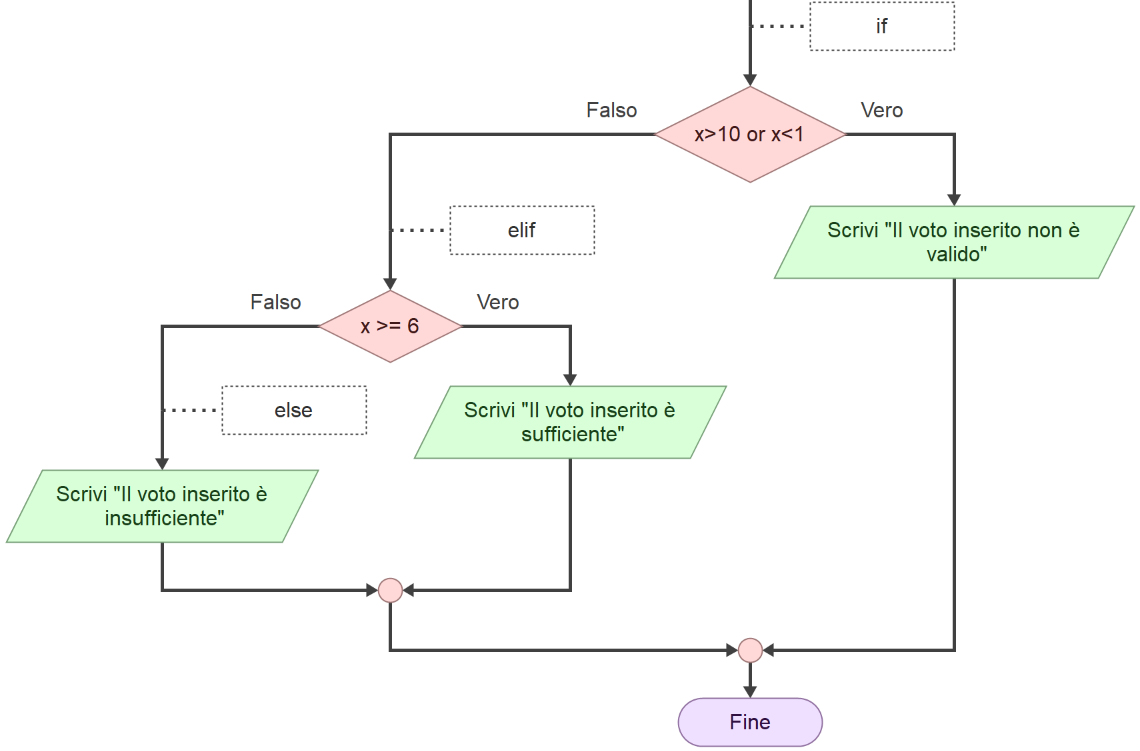
\includegraphics[width=.85\linewidth]{img/elif.png}
        \caption{{creata con \href{http://flowgorithm.org/}{Flowgorithm}}}
    \end{figure}
\end{frame}

\section{ISTRUZIONE MATCH CASE}

\begin{frame}[fragile]{ISTRUZIONE MATCH CASE}
    \begin{alertblock}{DEFINIZIONE}
        \begin{minipage}{0.98\linewidth}
            \justifying
            L'istruzione \textbf{match casemm} permette di selezionare un blocco di codice tra molti 
            in base al contenuto di una variabile (invece che concatenare molti elif).\\
            Il \textbf{case \_} è opzionale e viene utilizzato per eseguire un blocco di codice nel 
            caso in cui non avvenga alcun match.
\begin{lstlisting}[language=Python]
 match status:
    case 404:
        print("Not Found")
    case 200:
        print("OK")
    case 500:
        print("Internal Server Error")
    case _:
        print("Codice non classificato")
\end{lstlisting}
        \end{minipage}
    \end{alertblock}
\end{frame}

\section{}

\end{document}